%% APPENDIX A -- spectral response, frequency conventions, primary-beam response.
%% Owner: appendix-triage.  Carries \label{app:conventions} (cited by
%% 04_method.tex) and \label{app:pbresp}.
\section{Spectral response, frequency conventions and the primary-beam
response}
\label{app:conventions}

A reader checking a threshold in this paper needs three things: the frame
every frequency is quoted in, the instrumental response that separates a
channel threshold from a transmitter power, and the primary-beam factor that
converts a measured noise into a flux at the star. They are collected here.
The per-window catalogue, \texttt{catalogue/windows.csv} in the deposit,
carries one row per searched window and the columns each of these corrections
uses.

\begin{figure*}
\centering
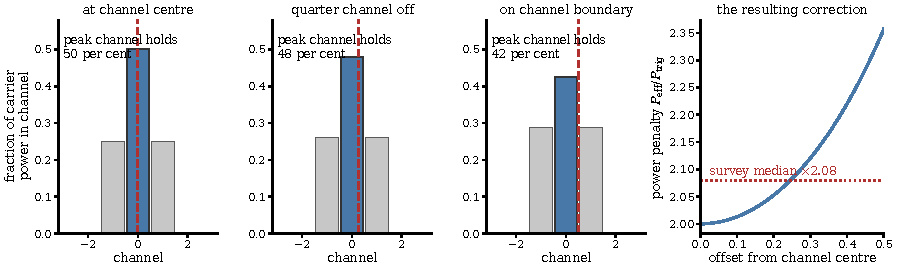
\includegraphics[width=0.94\textwidth]{figures/hanning_response.pdf}
\caption{Why the nominal channel threshold is not the transmitter
threshold. ALMA applies online Hanning smoothing by default, so an
intrinsically unresolved carrier is spread over neighbouring channels and
the peak channel holds only part of its power: half at a channel centre,
\HanWorst{} on a boundary (first three panels; blue is the peak channel,
the dashed line the carrier). The search threshold is set in units of the
channel noise, so the power a transmitter must radiate to reach it is
larger than the nominal figure by the reciprocal of that fraction
(right-hand panel). This is the whole of the difference between
$P_{\rm trig}$ and $P_{\rm eff}$.}
\label{fig:hanning}
\end{figure*}

\subsection{Frequency frames, linewidth and smearing}
%% (subsection label retired: nothing cites it)

Every frequency axis here --- searched spectra, tabulated ranges and
crossing frequencies alike --- is \emph{topocentric} as delivered by the
ALMA correlator, and the search itself applies no velocity-frame shift.
Velocities enter at the vetting stage, where the line mask is evaluated in
each star's own rest frame: it carries every crossing frequency to the
barycentre at its own block's epoch and then to the stellar frame before
comparing it with a transition (Appendix~\ref{app:linemask}). The residual
error is then the catalogue radial-velocity uncertainty alone, a few
km\,s$^{-1}$ within 40\,pc; second-order relativistic terms at the
\MaskHalfKms\,km\,s$^{-1}$
scale are $\lesssim5$\,kHz at 350\,GHz, below the finest native channel
searched. The stacking is drift-aligned and inverse-variance weighted:
coherent in frequency trajectory, not in electric-field phase.

The native channel width is also the linewidth convention for every EIRP
threshold. Channel dilution spreads a sub-channel carrier's total flux
across the channel, so EIRP$_{\rm trig}$ is the minimum \emph{total} power
of a channel-confined carrier, independent of the transmitter's own width
below the channel, and never a spectral power density. The Hz-resolution
surveys' limits are total powers in the same sense, each the best case of
its own channelisation, which makes the axes of Fig.~\ref{fig:context}(a)
commensurable. One number fixes the scale, illustratively and not
achievably: the median Class~A channel is \SqrtScaleChanKHz\,kHz, so
rechannelising the same data to the \SETIChanHz\,Hz of a dedicated
narrowband search would, on $P_{\min}\propto\sqrt{\Delta\nu}$, divide the
threshold by $\SqrtScaleFac$. ALMA cannot do this: the correlator delivered the
channelisation the archive holds, and no reprocessing recovers resolution
that was never recorded.

Channel widths come from the measurement sets' own spectral window tables
(CHAN\_WIDTH). A missing ``EFFECTIVE\_BANDWIDTH'' column is not evidence of
an absence of online spectral averaging, MS~v2 defining no such column, so
the quoted channelisations are not claimed to be noise bandwidths.

ALMA applies online Hanning smoothing by default, so the spectral response
is ${\sim}2$ channels wide and neighbouring channels are correlated
(Fig.~\ref{fig:hanning}). For the $0.25/0.5/0.25$ kernel the coefficients
are $\rho_1=\HanRhoOneFrac=\HanRhoOne$ and $\rho_2=\HanRhoTwo$, with
$\sigma_{\rm smoothed}/\sigma_{\rm raw}=\HanSigRatio$: the correlation is
not confined to adjacent channels, the lag-two term being a sixth. The
peak-channel fractions \HanWorst--\HanBest, median \HanMed, and the
resulting $\times\HanFacBest$--$\times\HanFacWorst$ optimism of a nominal
threshold are given in \S\ref{sec:method}; the released catalogue carries the
nominal threshold and both corrected values for every window.

\emph{The injected carriers are deposited with the correlator's own channel
response, at a sub-channel phase drawn afresh for each tone, so the smoothing
loss sits inside the measured completeness rather than being applied to it.}
The deposited profile is the tone divided between the two channels it
straddles and then passed through the three-point kernel, which leaves
\InjDepCentre{} of the flux in the peak channel for a carrier at a channel
centre and \InjDepEdge{} for one on a boundary, against \InjRespEdge{} for
the exact transform of the lag window; averaged over phase the deposition
therefore falls \InjShortPct{} per cent short of the ideal response, and the
completeness is conservative by that much. Where in a channel a carrier was
placed makes no difference to its recovered signal-to-noise: the medians over
\InjNPhaseTone{} tones agree across the whole range of sub-channel phase to
\InjPhaseFlatPct{} per cent, because a carrier at a typical searched drift
rate crosses about \InjDriftChan{} channels during one observation and so
samples the whole response. Since the loss is carried end to end it must not
be applied to the result as well: at the ninety per cent point of the
recovery curve the peak channel holds $\InjPeakAtNinety\times$ the nominal
trigger flux, which is that factor of about two, already spent.

Two measurements fix the smoothing state. The retained per-integration
residuals of the second-stage local null have a lag-one spectral
autocorrelation of \LNLagOne{} against the Hanning prediction \HanRhoOne, so
the correlation is instrumental and those spectra are smoothed and
un-averaged; and the archive's reported effective spectral resolution is
exactly twice the channel separation in \NHanTwo{} of the \NHanKnown{}
windows, in both correlator modes. The other \NHanOther{} report a smaller
ratio, the signature of online channel averaging, where the peak-channel loss
is smaller, and the \NNoArchRes{} Band~9 and~10 windows absent from the
metadata snapshot take ALMA's default, so the blanket factor is right for the
great majority of both classes. \emph{The correlation model is truncated at
lag two}: the baseline step, a per-integration median in blocks of up to
\MedWin{} channels, could imprint correlation on longer scales that the
released products retain no residual spectra to measure, which would make the
independent-trials count of Appendix~\ref{app:falsealarm} an over-estimate.

\emph{Linewidth convention.} The statistic is the single-channel flux
density after drift correction, so the quoted EIRP$_{\rm trig}$ applies to
any transmitter narrower than the native channel and is flat in the assumed
linewidth. Flatness is exact only for a centred tone; a boundary-straddling
one divides its power between two channels, which is the loss the injections
carry and the reason EIRP values are quoted to two significant figures.

\emph{Transmitters wider than one channel.} The baseline filter
(\S\ref{sec:statistic}) is flat for features narrower than roughly half its
effective width $W$ and falls to zero above $W$, so the survey's sensitivity
is to channel-confined morphologies and $W$ is the linewidth ceiling:
\MedWinFineLo--\MedWinFineHi{} channels over the fine class and
\MedWinCoarseLo--\MedWinCoarseHi{} over the coarse one, that is
${\approx}\MedWinCeilFineMHz$\,MHz at \ChanFineKHz\,kHz and
${\approx}\MedWinCeilCoarseGHz$\,GHz at \ChanCoarseMHz\,MHz. Within that
ceiling, a top-hat transmitter spanning $N_{\rm ch}$ native channels has
per-channel flux the total divided by $N_{\rm ch}$ at unchanged noise, so to
first order
\begin{equation}
\mathrm{EIRP}_{\rm trig}(N_{\rm ch}) \;\simeq\; N_{\rm ch}\times
\mathrm{EIRP}_{\rm trig}(1), \qquad N_{\rm ch} \lesssim W/2,
\end{equation}
the rescaling the main text applies to signals broader than one channel.

\emph{Intra-integration smearing.} The frequency excursion at the maximum
searched drift rate across one integration is at most 1.10 channels over the
\NWindows{} windows, and a drift smeared by $\Delta$ channels within an
integration keeps $\eta_{\rm smear}=\mathrm{sinc}(\pi\Delta/2)$ of the peak
amplitude, so the effective threshold is
$\mathrm{EIRP}_{\rm trig}/\eta_{\rm smear}$. Only \NSmearLo{} windows have
$\eta_{\rm smear}<0.99$ --- \SmearList{} --- and the remaining \NSmearOk{}
agree with their nominal thresholds to better than one per cent. Compounding
the worst smearing penalty with the worst Hanning factor gives
$\times\CompoundWorst$ for those few, a product no released column carries.

\subsection{The primary-beam response, and the two columns that let a reader
recompute it}
%% (subsection label retired: nothing cites it)

The sensitivity quoted for a window is $S_{\min}=5\sigma/A$, where $A$ is the
primary-beam response at the star's offset from the phase centre: the noise
$\sigma$ is measured in apparent flux, the limit is quoted in true flux, and
the two differ by $A$. That offset is not a nuisance. Archival fields are
pointed at a catalogue position, often decades old, while these are
high-proper-motion stars, so the star can sit well off axis: over the
\PbNWin{} released windows the offset has a median of \PbOffMed$''$, a 99th
percentile of \PbOffPNN$''$ and a maximum of \PbOffMax$''$, and $A$ runs from
\PbAMed{} in the median down to \PbAMin, below $0.99$ on \PbNLowNN{} windows
and below $0.9$ on \PbNLowN. \emph{None} falls below one half, and every one
of the low-response windows is a physically explicable J2000 pointing on a
fast-moving star rather than an error. A window is kept only where the
response is at least \PbFloorResp, a correction of at most
$\times\PbFloorCorr$, since at low response a small error in the beam model
becomes a large error in inferred flux. The offsets are bimodal and the floor
sits in the gap: the last retained window has response \PbGapKeptResp{} at
$\PbGapKeptU\,\theta_{\rm PB}$, the first window beyond it \PbGapHeldResp{}
at $\PbGapHeldU\,\theta_{\rm PB}$, and nothing lies between, so the rule
binds prospectively and excludes none of the \NWindows{} released windows.
Beyond it are the \EpsEriNWin{} $\epsilon$\,Eri Band~6 windows at
$\EpsEriPbLo$--$\EpsEriPbHi\times$, also past the first sidelobe transition
where the Gaussian form fails; the two criteria are independent and select
the same windows. They are \emph{withheld}, enter no number here and are
absent from the released catalogue, although under the nominal rule they
would have covered $\EpsEriEirpLo$--$\EpsEriEirpHi$\,W at \EpsEriDistPc\,pc.

\emph{The correction is applied exactly once, and that is the complete
correction.} The offset is computed for every measurement set from its own
\texttt{FIELD::PHASE\_DIR} and the propagated stellar position, so no window
carries a zero-by-assumption offset. It enters the published numbers in one
place only: the identity $S_{\min}=5\sigma/A$ closes on all \PbSminClosed{}
released rows to \PbSminWorstRes{} in relative terms. \emph{The count is
given in two parts, because on part of it the identity cannot fail}: on
\PbSminTaut{} rows whose products are not retained $A$ is back-solved from
$5\sigma/S_{\min}$ and is flagged as such in the catalogue, so there the
closure is arithmetic and shows it, at \PbSminTautRes{} against
\PbSminIndepRes{} on the \PbSminIndep{} rows where $A$ comes from the
search's own stored geometry. \PbSminIndep{} is therefore the number of rows
on which the audit is a test. Nothing else needs correcting, because the
detection statistic of Eq.~\ref{eq:tstar}, the control ranks and the
attribution are all \emph{ratios} formed inside a single window, in which $A$
divides out identically; no crossing, no rank and no disposition depends on
it.

Two catalogue columns, \texttt{pb\_offset\_arcsec} and \texttt{pb\_atten},
carry the offset and the response per window so that a reader can repeat the
calculation. They are needed, because the only other geometry column,
\texttt{theta\_pb\_arcsec}, is the pipeline's $1.22\lambda/D$ evaluated at
$D=12$\,m for \emph{every} window --- including the \PbNAcaRow{} rows taken
on the \PbAcaRatio$\times$ smaller ACA dishes, where it is correspondingly
too narrow --- so recomputing $A$ from it alone would give the wrong answer
on the majority of the catalogue. The annulus geometry keeps the pipeline's
own $\theta_{\rm PB}=\RingPbCoefCode\,\lambda/D$, an Airy first-null
coefficient; recomputing it on ALMA's FWHM $\RingPbCoef\,\lambda/D$ at each
window's own dish diameter moves \NPbFixOnePct{} of \NWindows{} windows by
more than 1 per cent, extremes $\PbFixLoPct$ to $+\PbFixHiPct$ per cent, and
no headline threshold moves.

\emph{The beam model itself is a bounded systematic, and it is bounded by
measurement.} \texttt{pb\_atten} reproduces the Gaussian at $1.22\lambda/D$
that the pipeline applied; CASA's blocked-Airy response is the better
physics. Evaluated window by window, the largest ratio between the two over
the whole release is \PbModelMax, and the counts of systems reaching
$10^{15}$\,W are identical under either model.

\emph{The injection campaign is blind to $A$ by construction, and the
resulting bias is exactly zero.} The injector deposits an unattenuated
amplitude at the star's own direction cosines, which would bias the measured
completeness if the ladder were calibrated in true flux --- and it is not. On
all \PbInjNUnit{} scored units the ladder is referred to the \emph{apparent}
$5\sigma$, so an injected apparent amplitude recovered nine times in ten
implies a true flux larger by $1/A$ while $P_{\rm trig}$ is the power of a
true $5\sigma/A$, and $A$ cancels identically; \PbInjNDistinct{} of the
\PbInjNUnit{} units have apparent and corrected $S_{\min}$ differing by more
than a part in a thousand, so the cancellation is tested and not vacuous. Two
limitations remain. Being self-consistent in apparent flux, \emph{the
campaign can never falsify the beam model}; and injected configurations span
\PbInjOffMin$''$ to \PbInjOffMax$''$ (median \PbInjOffMed$''$,
$A\ge\PbInjAMin$) whereas \PbNBeyond{} released windows on \PbNBeyondStar{}
stars lie further out, reaching $A=\PbBeyondAMin$, so for those the
completeness is \emph{interpolated rather than measured}. Their
\PbNBeyondCross{} crossings are ratios and unaffected, but a limit quoted for
one of those stars rests on an extrapolated curve.

\emph{Four rows carry a published noise that no retained product
reproduces}, and they are declared rather than reconciled: \PbGapN{} windows
of \PbGapStar{} in execution block \texttt{\PbGapEb}, whose published
$\sigma$ is \PbGapPctLo--\PbGapPctHi{} per cent \emph{higher} than the
surviving product's, so the published limits there are weaker and not
stronger. With the \PbGapNoProd{} windows whose products are not retained at
all, the declared provenance gap is \PbGapDeclared{} windows. The two
attenuation columns are unaffected: for these rows $A$ comes from a retained
product at the same position, where $A\ge\PbGapAMin$, and
$S_{\min}=5\sigma/A$ still closes to \PbGapSminRes.

%% ------------------------------------------------------------------
%% REQUEST (appendix-triage -> integrator / 08_backmatter owner):
%%   \label{app:repro} no longer exists.  08_backmatter.tex cites it in the
%%   Data Availability statement.  Repoint that sentence at
%%   \ref{app:conventions}, or better, drop the cross-reference and name the
%%   deposit directly -- the sentence is about the release, not an appendix.
%% REQUEST (appendix-triage -> numbers):
%%   The UV Ceti worked example (flux -> EIRP) was deleted from this appendix
%%   because two of its four numbers are typed literals with no macro
%%   (1.21e-29 W/m2/Hz and 1.6e13 W).  If a worked example is wanted back,
%%   three macros are needed: the flux density, the implied EIRP and the
%%   distance used.  It is the clearest single verification aid in the paper.
%% REQUEST (appendix-triage -> stack-discussion, Section 6):
%%   The transmitter-power benchmark was deleted here.  Exactly one benchmark
%%   should survive, in Section 6: a \BenchDiam-m aperture radiating 1 MW at
%%   230 GHz, aperture efficiency 0.7, giving EIRP \BenchEirpSeven W, which
%%   the median Class A effective threshold \PeffWinMedA W misses by a factor
%%   \BenchEffRatio.  Macros \BenchDiam, \BenchGainSeven, \BenchEirpSeven,
%%   \BenchEffRatio, \PeffWinMedA and equation eq:gain are otherwise
%%   unreferenced and will be retired.  The Arecibo scale and the
%%   frequency-scaled Arecibo figure are deliberately not carried forward.
%% ------------------------------------------------------------------
